\documentclass[11pt,a4paper]{article}

% ==================== Packages ====================
\usepackage[utf8]{inputenc}
\usepackage[T1]{fontenc}
\usepackage{graphicx}
\usepackage{amsmath,amssymb}
\usepackage{booktabs}
\usepackage{multirow}
\usepackage[hidelinks]{hyperref}
\usepackage{geometry}
\usepackage{xcolor}
\usepackage[section]{placeins}
\geometry{left=2.5cm,right=2.5cm,top=2.5cm,bottom=2.5cm}
\newcommand{\figureplaceholder}[2]{%
  \fbox{\begin{minipage}[c][#1][c]{0.92\linewidth}\centering
  \textit{Figure placeholder: #2}\end{minipage}}}

\title{\textbf{ForenX-Bench: Auditing Cross-Dataset Reliability and Replayability in Image Manipulation Detection}}

\author{Author and affiliation details omitted from this public draft}
\date{}

\begin{document}
\maketitle

\begin{abstract}
Image manipulation detectors are commonly compared using classification and localization scores, although these metrics alone do not show how performance changes across datasets, post-processing conditions, or repeated executions. We present ForenX-Bench, an auditable evaluation protocol instantiated with two frozen localization models, TruFor and MVSS-Net, on Columbia Uncompressed, corrected CASIA v1, and corrected COVERAGE. The evaluation includes clean-image detection, mask-based localization where reference masks are dimensionally valid, controlled JPEG recompression and resize--restore stress tests, and hash-checked independent-process replay. Across the three datasets, image-level ROC-AUC ranged from 0.9958 to 0.7675 for TruFor and from 0.9752 to 0.7385 for MVSS-Net, showing dataset-dependent changes under a fixed 0.5 decision threshold. On CASIA v1, localization also varied by manipulation type, with copy-move F1 below splicing F1 for both models. For the replay audit, 90 stratified CASIA cases per model were independently rerun; all 180 runs reproduced scores and localization maps within an absolute tolerance of $10^{-5}$ after source-hash verification. These results establish deterministic replay in the tested software and hardware environment, but not cross-machine reproducibility, causal attribution, or forensic admissibility. ForenX-Bench provides code, manifests, aggregate results and replay records to support transparent extension of this evaluation; original datasets and model weights remain governed by their respective access and licensing terms.

\vspace{0.3em}
\noindent\textbf{Keywords:} image manipulation detection, digital image forensics, cross-dataset evaluation, robustness, reproducibility, auditability
\end{abstract}

\section{Introduction}

Image manipulation detection is increasingly evaluated as a supervised prediction task: a model assigns an authenticity score and, in localization settings, produces a pixel-level map. Such measurements are necessary for comparing systems, but their interpretation depends on the evaluation data and operating conditions. Dataset-specific acquisition and editing traces, annotation conventions, and post-processing can all affect the measured result. For forensic use, a high score on one benchmark should therefore not be read as evidence of stable performance on another dataset or after an image has been transformed.

This concern is visible in the broader image-forensics literature. Methods have progressed from analyses of acquisition and compression traces to learned image-level detectors and localization systems, including approaches based on self-consistency, rich manipulation features, and diffusion priors \cite{farid2009imageforgery,verdoliva2020mediaforensics,huh2018fighting,zhou2018rich,wu2019mantra,yu2024diffforensics}. Newer benchmarks broaden the range of synthetic-image and manipulation sources \cite{ojha2023universal,yan2024df40,zhu2023genimage,du2025forensichub}. Yet benchmark scores are not directly interchangeable when dataset composition, reference-mask meaning, model thresholds, or image processing differ. A reliable evaluation should report those conditions alongside the scores and should retain enough provenance to verify which inputs and model outputs produced each reported result.

Two further questions remain relevant after an evaluation has been run. First, how sharply do detection and localization results change across independent datasets and controlled post-processing? Second, can the reported model outputs be regenerated from the same source files and frozen model artifacts in a separate process? Standard detection metrics answer neither question by themselves. Forensic guidance emphasizes documented methods, observations and limitations, while benchmark initiatives emphasize performance under varied operational conditions \cite{swgde2025imageauth,nist2025guardians,nistopenmfc}. In this study, we treat evidence auditability narrowly as record completeness, input-integrity verification and deterministic output replay. These properties support technical inspection; they do not establish causal attribution or legal admissibility.

We present ForenX-Bench as an auditable evaluation protocol and report its completed instantiation using frozen TruFor and MVSS-Net models on Columbia Uncompressed, corrected CASIA v1 and corrected COVERAGE. The study evaluates image-level detection and mask-based localization under a fixed threshold, applies JPEG recompression and resize--restore stress transformations, and records model inputs and derived outputs in machine-readable manifests. A seeded, manipulation-stratified sample is then rerun in an independent process with input hashes checked and numerical agreement assessed at a predeclared tolerance. We ask whether performance is consistent across these datasets and transformations, where mask-based comparisons require annotation-specific qualifications, and whether the retained outputs can be reproduced under the recorded execution conditions.

The contribution is an empirical, reproducible audit of existing detectors rather than a new detection architecture. Specifically, we (i) report cross-dataset detection and localization results for two frozen models across three manipulation datasets; (ii) quantify changes under controlled JPEG and resize--restore transformations without retuning the decision threshold; and (iii) provide an auditable evidence record with a stratified independent-process replay assessment. The scope is limited to the evaluated datasets, checkpoints, transformations and execution environment. A dual-branch detector pilot is retained as a supplementary negative result and is not presented as evidence of an algorithmic improvement.

\section{Related Work}

\subsection{Image manipulation detection and localization}
Image-forensics methods exploit inconsistencies in acquisition, compression, noise, and editing traces, while learned approaches estimate manipulation scores or suspicious regions directly from image content \cite{farid2009imageforgery,verdoliva2020mediaforensics}. Research has addressed splice detection through learned self-consistency and rich manipulation features, and later systems have combined anomaly cues with deep localization architectures \cite{huh2018fighting,zhou2018rich,wu2019mantra,yu2024diffforensics}. MVSS-Net uses noise-sensitive and boundary-artifact views with multi-scale supervision, whereas TruFor fuses high- and low-level clues and outputs image-level integrity scores and localization maps \cite{chen2021mvss,guillaro2023trufor}. These systems motivate our choice of two frozen detectors with different designs. Our study does not retrain either method or propose a competing architecture; it measures how their released implementations behave under a common evaluation protocol.

\subsection{Benchmark data and evaluation scope}
Public datasets provide complementary but non-equivalent evaluation conditions. Columbia Uncompressed isolates splicing in uncompressed images and includes a dataset-specific reference annotation; CASIA provides authentic and manipulated examples spanning splicing and copy-move; COVERAGE was designed for copy-move forgery evaluation \cite{hsu2006columbia,dong2013casia,wen2016coverage}. Their source composition, image processing and annotation semantics differ. Accordingly, aggregate pixel scores should be interpreted with the provenance and validity of each reference mask in view. Generalization-focused synthetic-image detectors and broader benchmarks such as GenImage and DF40 study a related but distinct image-authentication problem, while ForensicHub addresses a wider set of image-forensics tasks \cite{ojha2023universal,zhu2023genimage,yan2024df40,du2025forensichub}. The present study is restricted to local image manipulation and the three named datasets.

\subsection{Explainability, audit records and reproducibility}
General attribution techniques such as LIME, Integrated Gradients, SHAP and Grad-CAM explain model outputs through feature relevance or saliency estimates \cite{ribeiro2016lime,sundararajan2017axiomatic,lundberg2017unified,selvaraju2017gradcam}. Recent systems extend image-forgery detection with multimodal explanations, textual rationales and localization, including FakeShield, SIDA and X2-DFD \cite{xu2024fakeshield,huang2025sida,chen2025x2dfd}. Such work makes explanation outputs available for inspection, while reproducibility of a prediction is a separate property: it requires identification of the input, model artifact, execution settings and derived output, together with a procedure for replay.

Digital-evidence guidance emphasizes documenting methods, findings and limitations, and forensic evaluation initiatives consider performance in operationally relevant settings \cite{swgde2025imageauth,nist2025guardians,nistopenmfc}. Broader discussions of AI in digital forensics and validation of forensic evaluation methods similarly motivate explicit scope and error characterization \cite{casey2022digitalforensics,ramos2017lrvalidation}. ForenX-Bench operationalizes a limited technical audit around these concerns: it records the evaluated artifacts and conditions, verifies source hashes, and tests deterministic replay in an independent process. It does not test examiner performance, validate a legal opinion, or equate reproducible output with causal evidence.

\section{ForenX-Bench Evaluation Set-up}
\FloatBarrier

\subsection{Datasets and annotation scope}
We evaluated three existing image-manipulation datasets without redistributing their source files. Columbia Uncompressed contributes 363 images (183 authentic and 180 spliced). The provided blue-region annotation is specific to the dataset's splice-boundary/camera-region convention and is not treated as a general complete tampered-area mask. Corrected CASIA v1 contributes 1,721 images (800 authentic and 921 tampered); 920 tampered images have dimension-aligned pixel masks. Corrected COVERAGE contributes 200 images in 100 authentic--tampered pairs; 91 tampered images have masks dimensionally aligned with their image. All 200 COVERAGE images are retained for detection, while the nine mismatched masks are excluded only from localization. The dataset sources and annotation denominators are summarized in Table~\ref{tab:datasets}.

\begin{table}[t]
\centering
\caption{Evaluation data and valid annotation scope. Counts refer to the corrected local dataset bundles used in this study. Columbia reference annotations have dataset-specific semantics and must not be interpreted as complete manipulation masks.}
\label{tab:datasets}
\small
\resizebox{\textwidth}{!}{%
\begin{tabular}{lrrrrl}
\toprule
Dataset & Authentic & Manipulated & Detection $n$ & Valid masks & Manipulation type \\
\midrule
Columbia Uncompressed & 183 & 180 & 363 & 180$^*$ & Splicing \\
CASIA v1 corrected & 800 & 921 & 1,721 & 920 & Splicing, copy-move \\
COVERAGE corrected & 100 & 100 & 200 & 91 & Copy-move \\
\bottomrule
\end{tabular}
}
\\[0.25em]
\parbox{\linewidth}{\footnotesize $^*$The Columbia reference has splice-boundary/camera-region semantics, so its pixel metrics are reported separately and are not directly comparable to complete manipulated-region masks.}
\end{table}

\subsection{Sample integrity and provenance}
Each evaluated input is identified by a dataset-relative sample identifier and a SHA-256 digest. Dataset manifests record the source bundle, class label, manipulation category where available, dimensions, mask availability and integrity information. Model outputs and stress derivatives are linked to the originating image through records that identify the model artifact and transformation parameters. The raw datasets and model weights remain outside the project archive; acquisition instructions and checksums support users in obtaining and validating their own copies under the upstream conditions.

\begin{figure}[t]
\centering
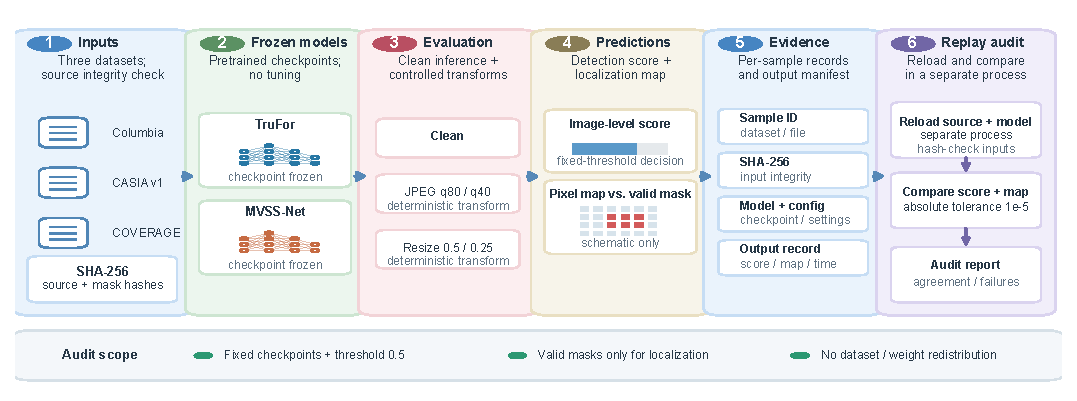
\includegraphics[width=\linewidth]{reports/figures/evaluation_workflow.pdf}
\caption{ForenX-Bench evaluation and audit workflow. Dataset files are integrity-checked before inference with frozen TruFor and MVSS-Net checkpoints. Clean and controlled transformed inputs are evaluated for image-level detection and mask-based localization where reference masks are valid. Sample-level records retain input identity, hashes, model/configuration information and outputs. A stratified subset is reprocessed independently and compared with stored outputs at an absolute tolerance of $10^{-5}$. The map and mask icons are schematic; datasets and model weights are not redistributed.}
\label{fig:workflow}
\end{figure}

\FloatBarrier
\subsection{Frozen model artifacts}
The evaluation uses released TruFor and MVSS-Net implementations and checkpoints without additional training or threshold tuning on the evaluation datasets \cite{guillaro2023trufor,chen2021mvss}. TruFor was executed at upstream code commit \texttt{ae54475d\allowbreak{}f6f41a49\allowbreak{}1d761510\allowbreak{}0feb1926\allowbreak{}3dec13f7}; the checkpoint MD5 recorded in the experiment provenance is \texttt{7bee48f3\allowbreak{}476c7561\allowbreak{}6c3c5721\allowbreak{}ab256ff8}. MVSS-Net used the authors' CASIAv2 checkpoint, recorded by SHA-256 \texttt{080bc6c3\allowbreak{}aae59f74\allowbreak{}8b547dbf\allowbreak{}090786fe\allowbreak{}9d31a6e5\allowbreak{}0749daaa\allowbreak{}40871e29\allowbreak{}8d6a7e50}. Both image-level and pixel-map decisions use a fixed threshold of 0.5. Since MVSS-Net was trained with CASIAv2 data and the locally reconstructed CASIA v1 set is not the official CASIAv1plus construction, potential source overlap limits interpretation of its CASIA result as fully independent.

\subsection{Controlled digital stress transformations}
For Columbia and CASIA v1, each original image was processed under four deterministic conditions: JPEG recompression at quality 80, JPEG recompression at quality 40, resize to 0.5 times followed by restoration to the original dimensions, and resize to 0.25 times followed by restoration. Transformation manifests preserve the condition and source-image link. These conditions probe sensitivity to compression and resolution loss; they do not model a named social platform, physical screen recapture, or every real-world processing chain. COVERAGE is used for clean-image detection and valid-mask localization in the current release, without the same four-condition pressure-test suite.

\subsection{Evidence records}
For every CASIA v1 image--model pair, the workflow writes one JSONL evidence record. Required fields include the bounded image-level prediction claim, image and output identifiers, source hash, frozen model identity, operation/configuration reference, output-file integrity data, and applicability and failure notes. This record is an auditable computational trace; it is not a human-authored forensic opinion and does not assert that a model cue uniquely identifies manipulation.

\section{Evaluation Protocol and Metrics}

\subsection{Detection and localization}
Image-level detection is evaluated using the continuous model score and binary labels. We report the area under the receiver-operating-characteristic curve (ROC-AUC) and, at the fixed threshold of 0.5, accuracy, precision, recall and F1. Pixel-level localization is evaluated only for images with a dimension-aligned reference mask. At the fixed pixel threshold of 0.5, we compute precision, recall, F1, intersection over union (IoU) and Matthews correlation coefficient (MCC) per image and macro-average across eligible images. Metrics are reported by manipulation subtype when subtype labels are available. Columbia's special reference convention is reported with an explicit semantic qualification.

\subsection{Evidence coverage and traceability}
Let $D$ be the set of valid image--model decisions, $E$ the set of emitted evidence records, and $E_c\subseteq E$ the records that contain all required provenance, model, operation and integrity fields. Evidence Coverage Rate (ECR) and Evidence Traceability Rate (ETR) are defined as
\begin{align}
\mathrm{ECR} &= \frac{|E|}{|D|}, \\
\mathrm{ETR} &= \frac{|E_c|}{|E|}.
\end{align}
ECR measures whether an evidence record exists for a decision; ETR measures completeness among emitted records. They are evaluated on all 1,721 CASIA v1 images for each of two models. Missing records are counted as coverage failures rather than silently removed from the denominator.

\subsection{Independent replay}
Let $S$ be the seeded replay sample and $S_r\subseteq S$ the cases for which the prescribed inference completes after reloading the source image and frozen model artifact in a separate process. Replay Success Rate (RSR) is
\begin{equation}
\mathrm{RSR}=\frac{|S_r|}{|S|}.
\end{equation}
Replay sampling is stratified by CASIA v1 class (authentic, copy-move and splicing), with 30 samples per class and model (90 per model; 180 attempts total; seed 20260929). A replay is successful only when the source SHA-256 agrees with the manifest and inference returns the required image-level score and localization map. The experiment reports a Wilson 95\% interval for each model's 90/90 replay rate.

For successful cases, Evidence-Grounding Agreement (EGA) is the fraction for which both the absolute score difference and the maximum absolute localization-map difference between the replay and stored record are no greater than $\epsilon=10^{-5}$:
\begin{equation}
\mathrm{EGA}=\frac{1}{|S_r|}\sum_{i\in S_r}\mathbb{I}\left[|s_i-\tilde{s}_i|\leq\epsilon\ \land\ \|M_i-\tilde{M}_i\|_{\infty}\leq\epsilon\right],
\end{equation}
where $s_i$ and $M_i$ are the stored score and map, and $\tilde{s}_i$ and $\tilde{M}_i$ are their replayed counterparts. This strict numerical criterion tests deterministic replay in the recorded environment; it is not a cross-platform equivalence criterion.

\subsection{Stress-test analysis}
Each transformed image is evaluated against its untransformed counterpart using the same frozen model and 0.5 threshold. We report ROC-AUC and detection F1 under each condition, localization macro F1 where valid masks are available, the mean change in image-level score, and the fraction of cases whose binary decision changes. Stress results are descriptive for the tested images and transformations. They are not interpreted as estimates of performance under all deployment shifts.

\subsection{Uncertainty and comparisons}
For reported metrics with bootstrap intervals, resampling is performed over images rather than pixels; paired model comparisons use the same sampled images for both models. The CASIA paired comparisons use 5,000 nonparametric bootstrap resamples, and single-model confidence intervals use 2,000 resamples as specified by the analysis scripts. Replay proportions use Wilson intervals. The replay tests characterize computational repeatability, whereas detection and mask metrics characterize agreement with dataset labels; neither should be used as a substitute for the other.

\section{Results}
\FloatBarrier

\subsection{Clean-image detection across datasets}
Table~\ref{tab:detection} reports clean-image performance at the fixed decision threshold. ROC-AUC decreased from Columbia Uncompressed to CASIA v1 and COVERAGE for both frozen models. TruFor's AUC was 0.9958, 0.9052 and 0.7675, respectively; MVSS-Net's was 0.9752, 0.8390 and 0.7385. Columbia therefore provides a comparatively favorable result for these checkpoints and should not be treated as a sufficient estimate of performance on the other datasets. The same ordering is not captured fully by AUC alone: at threshold 0.5, MVSS-Net's Columbia F1 was 0.7412 despite its AUC of 0.9752, reflecting 124 false positives among 183 authentic images.

\begin{table}[t]
\centering
\caption{Clean-image detection performance for the frozen models. F1 uses the fixed 0.5 image-score threshold; ROC-AUC is threshold-free.}
\label{tab:detection}
\small
\begin{tabular}{llrrr}
\toprule
Dataset & Model & Detection $n$ & ROC-AUC & F1 \\
\midrule
Columbia Uncompressed & TruFor & 363 & 0.9958 & 0.9861 \\
 & MVSS-Net & 363 & 0.9752 & 0.7412 \\
CASIA v1 corrected & TruFor & 1,721 & 0.9052 & 0.7926 \\
 & MVSS-Net & 1,721 & 0.8390 & 0.7492 \\
COVERAGE corrected & TruFor & 200 & 0.7675 & 0.5811 \\
 & MVSS-Net & 200 & 0.7385 & 0.6714 \\
\bottomrule
\end{tabular}
\end{table}

\begin{figure}[t]
\centering
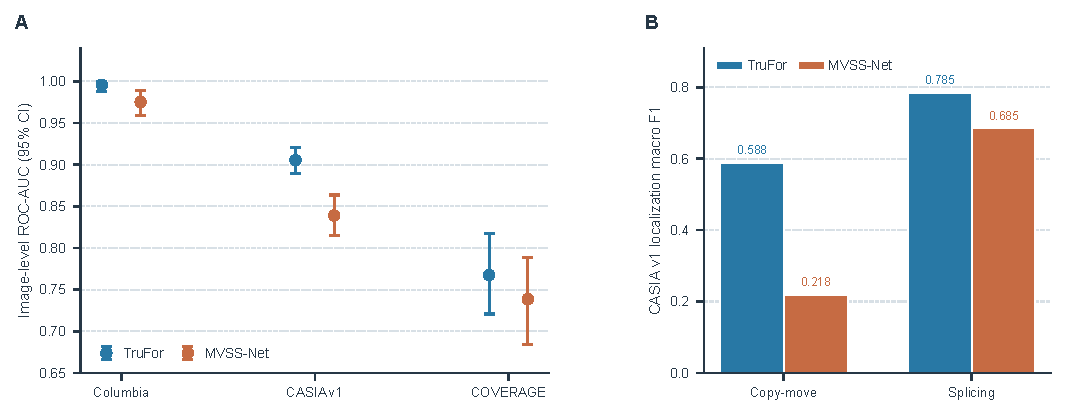
\includegraphics[width=\linewidth]{reports/figures/cross_dataset_comparison.pdf}
\caption{Cross-dataset detection and manipulation-type localization results. (A) Image-level ROC-AUC with dataset-specific 95\% bootstrap confidence intervals for Columbia Uncompressed ($n=363$), corrected CASIA v1 ($n=1{,}721$) and corrected COVERAGE ($n=200$). (B) CASIA v1 macro localization F1 by manipulation type, computed on valid reference masks (copy-move $n=459$; splicing $n=461$). Columbia confidence intervals use source-group bootstrap; CASIA and COVERAGE intervals use their prespecified bootstrap procedures.}
\label{fig:cross-dataset}
\end{figure}

On CASIA v1, the paired model difference in ROC-AUC was 0.0662 in favor of TruFor (95\% bootstrap CI 0.0462--0.0864; $p=0.0004$); the detection F1 difference was 0.0435 (0.0172--0.0695; $p=0.0012$). These paired comparisons are specific to the corrected CASIA v1 test bundle. Because the MVSS-Net checkpoint was trained on CASIAv2 and the local CASIA v1 bundle is not the authors' CASIAv1plus construction, possible authentic-content overlap remains a qualification on this comparison.

\subsection{Localization and manipulation-type differences}
Table~\ref{tab:localization} reports macro F1 on valid masks. Columbia results are listed for completeness but refer to overlap with its blue splice-boundary/camera-region annotation, not a complete tampered-area mask. CASIA and COVERAGE use manipulated-region references and are therefore the primary mask-localization comparisons. On CASIA, TruFor obtained higher overall F1 than MVSS-Net (0.6868 versus 0.4518); the paired difference was 0.2351 (95\% CI 0.2084--0.2614; $p=0.0004$). Both models localized splicing better than copy-move: TruFor F1 was 0.7854 versus 0.5879, while MVSS-Net F1 was 0.6848 versus 0.2177. The model-level average thus conceals a manipulation-specific performance gap.

\begin{table}[t]
\centering
\caption{Macro localization F1 on dimension-aligned reference masks. Columbia uses a dataset-specific boundary/source-region reference and should not be interpreted as directly comparable to complete tampered-region masks.}
\label{tab:localization}
\small
\begin{tabular}{llrr}
\toprule
Dataset / stratum & Model & Valid images & Macro F1 \\
\midrule
Columbia boundary reference & TruFor & 180 & 0.2613 \\
 & MVSS-Net & 180 & 0.2491 \\
CASIA v1, all tampering & TruFor & 920 & 0.6868 \\
 & MVSS-Net & 920 & 0.4518 \\
CASIA v1, copy-move & TruFor & 459 & 0.5879 \\
 & MVSS-Net & 459 & 0.2177 \\
CASIA v1, splicing & TruFor & 461 & 0.7854 \\
 & MVSS-Net & 461 & 0.6848 \\
COVERAGE, copy-move & TruFor & 91 & 0.5555 \\
 & MVSS-Net & 91 & 0.4817 \\
\bottomrule
\end{tabular}
\end{table}

\subsection{Sensitivity to compression and resizing}
The full-image stress tests applied JPEG recompression and resize--restore transformations to all Columbia and CASIA v1 images while keeping model weights and the 0.5 threshold fixed. Table~\ref{tab:stress} summarizes the clean condition, JPEG quality 40 and resize-to-0.25 condition. Results were transformation- and dataset-dependent. For example, TruFor's CASIA AUC fell from 0.9052 on clean images to 0.5923 after resize-to-0.25, while its Columbia AUC fell from 0.9958 to 0.8845. At the fixed threshold, CASIA TruFor F1 fell to 0.1583 and 34.40\% of binary decisions changed after the stronger resize. MVSS-Net also showed reduced AUC under stronger resizing, although the magnitude and thresholded F1 pattern differed by dataset. This variability cautions against treating one perturbation or one threshold-free metric as a general robustness certificate.

\begin{table}[t]
\centering
\caption{Selected full-image stress-test results. Each cell reports ROC-AUC / fixed-threshold detection F1. Flip rate is the fraction of image-level decisions changed from the clean prediction under resize-to-0.25.}
\label{tab:stress}
\small
\begin{tabular}{llrrr}
\toprule
Dataset & Model & Clean & JPEG q40 & Resize 0.25$\times$ \\
\midrule
Columbia & TruFor & 0.9958 / 0.9861 & 0.9861 / 0.8633 & 0.8845 / 0.8187 \\
 & MVSS-Net & 0.9752 / 0.7412 & 0.9642 / 0.7332 & 0.9057 / 0.7397 \\
CASIA v1 & TruFor & 0.9052 / 0.7926 & 0.8009 / 0.6612 & 0.5923 / 0.1583 \\
 & MVSS-Net & 0.8390 / 0.7492 & 0.6421 / 0.4855 & 0.6871 / 0.5402 \\
\midrule
Dataset & Model & \multicolumn{3}{c}{Flip rate at resize 0.25$\times$} \\
\midrule
Columbia & TruFor & \multicolumn{3}{c}{17.91\%} \\
 & MVSS-Net & \multicolumn{3}{c}{15.15\%} \\
CASIA v1 & TruFor & \multicolumn{3}{c}{34.40\%} \\
 & MVSS-Net & \multicolumn{3}{c}{31.67\%} \\
\bottomrule
\end{tabular}
\end{table}

Full metrics for all four stress transformations, including JPEG quality 80 and resize-to-0.5, are provided in Supplementary Table~\ref{tab:stress-complete}.

\begin{figure}[t]
\centering
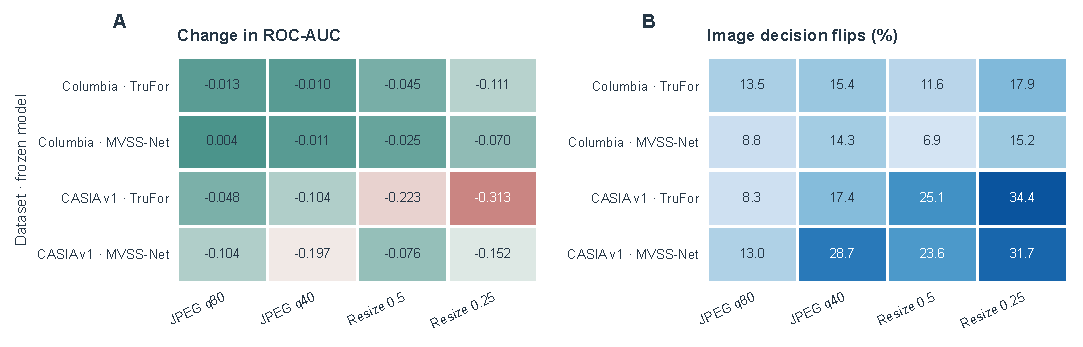
\includegraphics[width=\linewidth]{reports/figures/stress_sensitivity.pdf}
\caption{Sensitivity to controlled digital transformations. (A) Change in image-level ROC-AUC relative to the clean input for JPEG recompression (quality 80 and 40) and resize--restore (0.5 and 0.25 scale). (B) Image-level decision-flip rate relative to the clean prediction at the fixed 0.5 threshold. Rows identify dataset and frozen model; each Columbia condition includes 363 images and each CASIA v1 condition includes 1,721 images. Values are computed from the archived full-image stress summaries.}
\label{fig:stress}
\end{figure}

\subsection{Evidence completeness and independent replay}
For CASIA v1, one evidence record was generated for each of 1,721 images and two models (3,442 records total). ECR was 1.000 and ETR was 1.000. The independent-process replay sampled 90 cases per model, stratified evenly across authentic, copy-move and splicing classes. All source hashes matched and all 90 TruFor and 90 MVSS-Net cases reproduced both score and localization map within the absolute tolerance of $10^{-5}$; RSR and EGA were therefore 1.000 for each model. The Wilson 95\% interval was 0.959--1.000 for each 90/90 replay proportion. These results indicate complete records and deterministic replay in the tested environment. They do not show that every prediction is correct, that the model evidence is causally diagnostic, or that another machine will produce identical outputs.

The experiments also included handcrafted grayscale-statistics and ELA/logistic-regression baselines on a 73-image Columbia source-group test split. ELA reached ROC-AUC 0.8671 (95\% CI 0.6238--0.9701), compared with 0.8108 for grayscale statistics. These results use a smaller split; they are not paired against the frozen-model evaluation on 363 images.

\section{Discussion}

The evaluation shows why image-manipulation detector performance should be read jointly across datasets, thresholds and transformations. Both frozen models achieved their highest AUC on Columbia Uncompressed, while their AUCs were lower on corrected CASIA v1 and COVERAGE. Under the fixed 0.5 threshold, ranking quality and binary operating performance were not interchangeable: MVSS-Net's Columbia AUC was high, but its false-positive count on authentic images was also high. A single AUC therefore does not describe the decision behavior relevant to a specified operating threshold.

Localization results were also conditional on both manipulation type and reference-mask semantics. On CASIA v1, both models produced higher macro F1 for splicing than for copy-move manipulation, with a larger difference for MVSS-Net. On Columbia, the provided blue-region reference denotes a dataset-specific boundary/source-region convention rather than the complete edited object. Comparing an anomaly map to that reference measures spatial agreement with the provided annotation, not necessarily recovery of the full manipulated region. The dimension mismatch in nine COVERAGE masks similarly required those cases to be excluded from localization while retaining them for image-level detection. These distinctions should accompany any interpretation of the aggregate localization scores.

The controlled stress tests demonstrate sensitivity to post-processing in the tested samples. JPEG recompression and resize--restore affected the two datasets and models differently; strong resizing caused particularly large degradation for TruFor on CASIA v1. Since thresholds were fixed, these results expose changes in both score ordering and operating-point behavior. They do not establish the behavior of all detectors, social-media platforms, screen recapture, unseen cameras or future image-processing pipelines. The transformations are deterministic digital stress conditions, not a complete model of deployment distribution shift.

The evidence audit contributes a separate computational finding. Complete evidence records and successful independent-process replay show that the sampled predictions can be regenerated from hash-matched inputs and frozen artifacts under the recorded environment. Replay agreement does not imply prediction correctness, causal attribution, or diagnostic uniqueness. Nor does an independent process on the same host demonstrate cross-platform, cross-machine or third-party-laboratory reproducibility. No practitioner study was conducted, so no claim is made about improved human judgment, review time or report quality.

Several limits define the next validation steps. Only two pretrained models and three existing datasets were evaluated, and the potential overlap between the CASIAv2 training source and the corrected CASIA v1 bundle qualifies that comparison. The copy-move external evaluation in COVERAGE contains only 200 image-level cases, with 91 usable manipulation masks. Columbia's established status also means its high score should be interpreted as a known-benchmark replication rather than a wholly unseen-domain result. Future work should include additional independently sourced datasets, model versions, cross-machine replay, stronger split audits, and a preregistered examiner study before making broader operational claims. A small dual-branch training pilot is reported as supplementary negative evidence; it did not demonstrate a reliable external-domain gain and is not used to claim algorithmic novelty.

\section{Conclusion}
This study presents ForenX-Bench as an auditable evaluation protocol and applies it to two frozen image-manipulation localization models on Columbia Uncompressed, corrected CASIA v1 and corrected COVERAGE. Detection performance varied across datasets and under JPEG recompression and resize--restore transformations; CASIA v1 localization also differed substantially between splicing and copy-move cases. A hash-checked, stratified replay audit regenerated all 90 sampled outputs per model within the declared tolerance in the tested environment. These findings support reporting dataset-specific performance, annotation scope, transformation sensitivity and computational replay together. They do not establish a new detector, causal forensic evidence, cross-machine reproducibility or legal admissibility. The project files provide a reproducible starting point for further datasets, models and independent execution environments, subject to completion of the stated rights and release review.

\appendix
\section{Exploratory Dual-Branch Detector Pilot}
\setcounter{table}{0}
\renewcommand{\thetable}{S\arabic{table}}
\renewcommand{\theHtable}{S\arabic{table}}
This appendix records the algorithm-development pilot to keep its negative result available without presenting it as a contribution of the main study. A corrected source-connected CASIA v2 split was used for training and held-out testing; neither Columbia nor COVERAGE was used for training, fine-tuning or threshold selection. The pilot compared an RGB-only branch, a high-pass residual-only branch and a fused dual-branch network. The residual-only and fused variants used two seeds; the RGB-only result used one initial run. Table~\ref{tab:pilot} summarizes the held-out CASIA v2 and zero-shot external results.

\begin{table}[h]
\centering
\caption{Exploratory dual-branch pilot results (mean $\pm$ sample SD for two-seed variants). AUC is image-level detection; F1 is pixel-level localization. Columbia localization is omitted because its annotation has boundary/source-region semantics.}
\label{tab:pilot}
\small
\resizebox{\textwidth}{!}{%
\begin{tabular}{llrrr}
\toprule
Variant & Seeds & CASIA v2 AUC / F1 & COVERAGE AUC / F1 & Columbia AUC \\
\midrule
RGB-only & 1 & 0.8248 / 0.1454 & 0.5029 / 0.2081 & -- \\
Residual-only & 2 & 0.9779$\pm$0.0001 / 0.2738$\pm$0.0136 & 0.5016$\pm$0.0052 / 0.1545$\pm$0.0106 & 0.538$\pm$0.038 \\
Dual branch & 2 & 0.9745$\pm$0.0031 / 0.2468$\pm$0.0019 & 0.5018$\pm$0.0045 / 0.0901$\pm$0.0243 & 0.534$\pm$0.093 \\
\bottomrule
\end{tabular}
}
\end{table}

The dual-branch model did not improve on the residual-only model in these runs and was near chance on both external detection datasets. This pilot therefore does not support a new detector claim. Its limited seed count, fixed 20-epoch training budget and dataset-specific training source also preclude a broad comparative conclusion. The split construction, audit and full result files are documented in \texttt{reports/forenx\_dualbranch\_v2\_pilot.md} and the associated scripts and manifests.

\subsection{Complete digital stress-test results}
Supplementary Table~\ref{tab:stress-complete} lists clean-image performance and all four controlled transformation conditions for the two full-image stress datasets. Flip rate is measured relative to each model's clean-image decision on the same image.

\begin{table}[p]
\centering
\caption{Complete stress-test detection results. Values are image-level ROC-AUC, fixed-threshold F1 and decision-flip rate. All transformed evaluations retain the model weights and threshold of 0.5.}
\label{tab:stress-complete}
\scriptsize
\begin{tabular}{ll lrrr}
\toprule
Dataset & Model & Condition & ROC-AUC & F1 & Flip rate \\
\midrule
Columbia & TruFor & Clean & 0.9958 & 0.9861 & 0.00\% \\
 & & JPEG q80 & 0.9831 & 0.8683 & 13.50\% \\
 & & JPEG q40 & 0.9861 & 0.8633 & 15.43\% \\
 & & Resize 0.5$\times$ & 0.9513 & 0.8780 & 11.57\% \\
 & & Resize 0.25$\times$ & 0.8845 & 0.8187 & 17.91\% \\
 & MVSS-Net & Clean & 0.9752 & 0.7412 & 0.00\% \\
 & & JPEG q80 & 0.9789 & 0.7463 & 8.82\% \\
 & & JPEG q40 & 0.9642 & 0.7332 & 14.33\% \\
 & & Resize 0.5$\times$ & 0.9498 & 0.7426 & 6.89\% \\
 & & Resize 0.25$\times$ & 0.9057 & 0.7397 & 15.15\% \\
\midrule
CASIA v1 & TruFor & Clean & 0.9052 & 0.7926 & 0.00\% \\
 & & JPEG q80 & 0.8569 & 0.7126 & 8.31\% \\
 & & JPEG q40 & 0.8009 & 0.6612 & 17.43\% \\
 & & Resize 0.5$\times$ & 0.6826 & 0.4219 & 25.10\% \\
 & & Resize 0.25$\times$ & 0.5923 & 0.1583 & 34.40\% \\
 & MVSS-Net & Clean & 0.8390 & 0.7492 & 0.00\% \\
 & & JPEG q80 & 0.7351 & 0.5528 & 12.96\% \\
 & & JPEG q40 & 0.6421 & 0.4855 & 28.70\% \\
 & & Resize 0.5$\times$ & 0.7630 & 0.6881 & 23.65\% \\
 & & Resize 0.25$\times$ & 0.6871 & 0.5402 & 31.67\% \\
\bottomrule
\end{tabular}
\end{table}

\section*{Data Availability}
The Columbia Uncompressed dataset is available by request from the Columbia DVMM dataset page. The COVERAGE authors provide access through their repository and restrict use to non-commercial research. CASIA v1 images used here came from a third-party corrected distribution; the exact acquisition URL and terms were not preserved, so the image source and applicable terms must be independently verified before reuse. The CASIA v1 ground-truth repository is identified in the project data-rights statement. No original images, masks, per-image manifests, sample identifiers, hashes, or sample-level predictions are redistributed. Aggregate results and annotation-denominator details are available in the project repository. Users must obtain each dataset from a lawful source and follow current provider terms.

\section*{Code Availability}
The evaluation code, configurations, aggregate reports, and manuscript source are publicly available at \url{https://github.com/wunan-snsy/ForenX-Bench} (v1.0.0). The MIT License applies only to original project software code. Dataset files, annotations, upstream model implementations, checkpoints, and manuscript text are not covered by that software license. Per-sample manifests, hashes, evidence records, and replay logs are omitted because permission to publish those derived records was not verified. The repository's \texttt{DATA\_AND\_RIGHTS.md} and \texttt{data/SOURCES.csv} state the access routes and unresolved rights limits.


\section*{Acknowledgments}
Acknowledgment details omitted from this public draft.

\bibliographystyle{plain}
\bibliography{references}

\end{document}
